% !TeX spellcheck = en_GB
%%%%%%%%%%%%%%%%%%%%%%%%%%%%%%%%%%%%%%%%%%
%                                        %
%     Master thesis LaTeX template       % 
%  compliant with the SZJK regulations   %
%                                        %
%%%%%%%%%%%%%%%%%%%%%%%%%%%%%%%%%%%%%%%%%%
%                                        %
%  (c) Krzysztof Simiński, 2018-2022     %
%                                        %
%%%%%%%%%%%%%%%%%%%%%%%%%%%%%%%%%%%%%%%%%%
%                                        %
% The latest version of the templates is %
% available at                           %
% github.com/ksiminski/polsl-aei-theses  %
%                                        %
%%%%%%%%%%%%%%%%%%%%%%%%%%%%%%%%%%%%%%%%%%
%
%
% This LaTeX project formats the final thesis 
% with compliance to the SZJK regulations. 
% Please to not change formatting (fonts, margins,
% bolds, italics, etc).
%
% You can compile the project in several ways.
%
% 1. pdfLaTeX compilation
% 
% If you use the minted package for code snippets
% compile the project like this:
%
% pdflatex -shell-escape thesis
% biber                  thesis
% pdflatex -shell-escape thesis
% pdflatex -shell-escape thesis
%
% If you do not use the minted package, just comment 
% the package import \usepackage{minted} and its use in the thesis.
% Then run the compilation:
%
% pdflatex thesis
% biber    thesis
% pdflatex thesis
% pdflatex thesis
%
%
% 2. XeLaTeX compilation
%
% Compilation with the XeLaTeX engine inserts Calibri font
% in the title page. Of course the font has to be installed.
% As above you can use the minted package or not. 
% Compilation with the minted package:
%
% xelatex -shell-escape thesis
% biber                 thesis
% xelatex -shell-escape thesis
% xelatex -shell-escape thesis
%
% Without the minted package the compilation is simpler:
%
% xelatex thesis
% biber   thesis
% xelatex thesis
% xelatex thesis
%
%
% manuals for code snippets packages:
% https://ctan.org/pkg/minted
% https://ctan.org/pkg/listings
%
%%%%%%%%%%%%%%%%%%%%%%%%%%%%%%%%%%%%%%%%%%%%%%%%%%%%%%%%%%%%%%
% If you have any questions, remarks, just send me an email: %
%            krzysztof.siminski(małpa)polsl.pl               %
%%%%%%%%%%%%%%%%%%%%%%%%%%%%%%%%%%%%%%%%%%%%%%%%%%%%%%%%%%%%%%

%%%%%%%%%%%%%%%%%%%%%%%%%%%%%%%%%%%%%%%%%%%%%%%%%%%%%%%%%%%%%%%%%%%%%%%%%
% Please customise your thesis:
% TODO
\newcommand{\Firstnames}{Michał}
\newcommand{\Surname}{Dyla}
\newcommand{\Supervisor}{$\langle$dr inż. Tomasz Grzejszczak$\rangle$}
\newcommand{\Title}{Testing the level of chess game effectiveness depending on the type of used neural network}
\newcommand{\TitleAlt}{Thesis title in Polish}
\newcommand{\Program}{Control, Electronic, and Information Engineering}
\newcommand{\Specialisation}{Data Science}
\newcommand{\Id}{$\langle$274132$\rangle$}
\newcommand{\Departament}{$\langle$Department of Automatic Control and Robotics$\rangle$}


% If you have a consultant for your thesis, put their name below ...
\newcommand{\Consultant}{$\langle$mgr Eryka Probierz$\rangle$}
% ... else leave the braces empty:
%\newcommand{\consultant}{} % no consultant

% end of thesis customisation
%%%%%%%%%%%%%%%%%%%%%%%%%%%%%%%%%%%%%%%%%%


%%%%%%%%%%%%%%%%%%%%%%%%%%%%%%%%%%%%%%%%%%%%%%%
%                                             %
%    PLEASE DO NOT MODIFY THE FILE BELOW!     %
%                                             %
%%%%%%%%%%%%%%%%%%%%%%%%%%%%%%%%%%%%%%%%%%%%%%%



\documentclass[a4paper,twoside,12pt]{book}
\usepackage[utf8]{inputenc}                                      
\usepackage[T1]{fontenc}  
\usepackage{amsmath,amsfonts,amssymb,amsthm}
\usepackage[polish,british]{babel} 
\usepackage{indentfirst}



\usepackage{ifxetex}

\ifxetex
	\usepackage{fontspec}
	\defaultfontfeatures{Mapping=tex—text} % to support TeX conventions like ``——-''
	\usepackage{xunicode} % Unicode support for LaTeX character names (accents, European chars, etc)
	\usepackage{xltxtra} % Extra customizations for XeLaTeX
\else
	\usepackage{lmodern}
\fi



\usepackage[margin=2.5cm]{geometry}
\usepackage{graphicx} 
\usepackage{hyperref}
\usepackage{booktabs}
\usepackage{tikz}
\usepackage{pgfplots}
\usepackage{mathtools}
\usepackage{geometry}
\usepackage[page]{appendix} % toc,




\usepackage{csquotes}
\usepackage[natbib=true]{biblatex}
\bibliography{biblio/biblio}

\usepackage{ifmtarg}   % empty commands  

\usepackage{setspace}
\onehalfspacing


\frenchspacing

%%%%%%%%%%%%%%%%%%%%%%%%%%%%%%%%%%%%%%%%%%%%%%%%%%%%%%%%%%%%%%%%%%%%%
% listings
% packages: listings or minted
% % % % % % % % % % % % % % % % % % % % % % % % % % % % % % % % % % % 

% package listings
\usepackage{listings}
\lstset{%
language=C++,%
commentstyle=\textit,%
identifierstyle=\textsf,%
keywordstyle=\sffamily\bfseries, %\texttt, %
%captionpos=b,%
tabsize=3,%
frame=lines,%
numbers=left,%
numberstyle=\tiny,%
numbersep=5pt,%
breaklines=true,%
%morekeywords={descriptor_gaussian,descriptor,partition,fcm_possibilistic,dataset,my_exception,exception,std,vector},%
escapeinside={@*}{*@},% 
}

% % % % % % % % % % % % % % % % % % % % % % % % % % % % % % % % % % % 
% package minted
\usepackage{minted}

% This package requires a special command line option in compilation
% pdflatex -shell-escape thesis

%%%%%%%%%%%%%%%%%%%%%%%%%%%%%%%%%%%%%%%%%%%%%%%%%%%%%%%%%%%%%%%%%%%%%


%%%% TODO LIST GENERATOR %%%%%%%%%

\usepackage{color}
\definecolor{brickred}      {cmyk}{0   , 0.89, 0.94, 0.28}

\makeatletter \newcommand \kslistofremarks{\section*{Remarks} \@starttoc{rks}}
  \newcommand\l@uwagas[2]
    {\par\noindent \textbf{#2:} %\parbox{10cm}
{#1}\par} \makeatother


\newcommand{\ksremark}[1]{%
{%\marginpar{\textdbend}
{\color{brickred}{[#1]}}}%
\addcontentsline{rks}{uwagas}{\protect{#1}}%
}










%%%%%%%%%%%%%% END OF TODO LIST GENERATOR %%%%%%%%%%%  

%%%%%%%%%%%% FANCY HEADERS %%%%%%%%%%%%%%%
% brak kapitalizacji zywej paginy
\usepackage{fancyhdr}
\pagestyle{fancy}
\fancyhf{}
\fancyhead[LO]{\nouppercase{\it\rightmark}}
\fancyhead[RE]{\nouppercase{\it\leftmark}}
\fancyhead[LE,RO]{\it\thepage}


\fancypagestyle{onlyPageNumbers}{%
   \fancyhf{} 
   \fancyhead[LE,RO]{\it\thepage}
}

\fancypagestyle{noNumbers}{%
   \fancyhf{} 
   \fancyhead[LE,RO]{}
}


\fancypagestyle{PageNumbersChapterTitles}{%
   \fancyhf{} 
   \fancyhead[LO]{\nouppercase{\Firstnames \Surname}}
   \fancyhead[RE]{\nouppercase{\leftmark}} 
   \fancyfoot[CE, CO]{\thepage}
}
 



%%%%%%%%%%%%%%%%%%%%%%%%%%%







\newcounter{pagesWithoutNumbers}

%%%%%%%%%%%%%%%%%%%%%%%%%%% 
\usepackage{xstring}
\newcommand{\printOpiekun}[1]{%		

    \StrLen{\Consultant}[\mystringlen]
    \ifthenelse{\mystringlen > 0}%
    {%
       {\large{\bfseries CONSULTANT}\par}
       
       {\large{\bfseries \Consultant}\par}
    }%
    {}
} 
%
%%%%%%%%%%%%%%%%%%%%%%%%%%%%%%%%%%%%%%%%%%%%%%
 
% Please do not modify the lines below!
\author{\Firstnames\ \Surname}
\newcommand{\Author}{\Firstnames\ \MakeUppercase{\Surname}}
\newcommand{\Type}{MASTER THESIS}
\newcommand{\Faculty}{Faculty of Automatic Control, Electronics and Computer Science}
\newcommand{\Polsl}{Silesian University of Technology}
\newcommand{\Logo}{graf/politechnika_sl_logo_bw_pion_en.pdf}
\newcommand{\LeftId}{Student identification number}
\newcommand{\LeftProgram}{Programme}
\newcommand{\LeftSpecialisation}{Specialisation}
\newcommand{\LeftSUPERVISOR}{SUPERVISOR}
\newcommand{\LeftDEPARTMENT}{DEPARTMENT}

%%%%%%%%%%%%%%%%%%%%%%%%%%%%%%%%%%%%%%%%%%%%%%

 % Do not modify the settings.tex file.

% Add keywords for code snippets if you need
\lstset{%
morekeywords={string,exception,std,vector},% keyword for the listings package
}


%%%%%%%%%%%%%%%%%%%%%%%%%%%%%%%%%%%%%%%%   


\begin{document}
%\kslistofremarks 


%%%%%%%%%%%%%%%%%%%%%%%%%%%%%%%%%%%%%%%%%%%%%%%
%                                             %
%    PLEASE DO NOT MODIFY THE FILE BELOW!     %
%                                             %
%%%%%%%%%%%%%%%%%%%%%%%%%%%%%%%%%%%%%%%%%%%%%%%


%%%%%%%%%%%%%%%%%%  TITLE PAGE %%%%%%%%%%%%%%%%%%%
\pagestyle{empty}
{
	\newgeometry{top=1.5cm,%
	             bottom=2.5cm,%
	             left=3cm,
	             right=2.5cm}
 
	\ifxetex 
	  \begingroup
	  \setsansfont{Calibri}
	   
	\fi 
	 \sffamily
	\begin{center}
	\includegraphics[width=50mm]{\Logo}
	 
	
	{\Large\bfseries\Type\par}
	
	\vfill  \vfill  
			 
	{\large\Title\par}
	
	\vfill  
		
	{\large\bfseries\Author\par}
	
	{\normalsize\bfseries \LeftId: \Id}
	
	\vfill  		
 
	{\large{\bfseries \LeftProgram:} \Program\par} 
	
	{\large{\bfseries \LeftSpecialisation:} \Specialisation\par} 
	 		
	\vfill  \vfill 	\vfill 	\vfill 	\vfill 	\vfill 	\vfill  
	 
	{\large{\bfseries \LeftSUPERVISOR}\par}
	
	{\large{\bfseries \Supervisor}\par}
				
	{\large{\bfseries \LeftDEPARTMENT\ \Departament} \par}
		
	{\large{\bfseries \Faculty}\par}
		
	\vfill  \vfill  

    	
    \printOpiekun{\Consultant}
    
	\vfill  \vfill  
		
    {\large\bfseries  Gliwice \the\year}

   \end{center}	
       \ifxetex 
       	  \endgroup
       \fi
	\restoregeometry
}
  
  % Please to not modify the titlepage.tex file!

\cleardoublepage
 
\rmfamily\normalfont
\pagestyle{empty}

  

% TODO
\subsubsection*{Thesis title}  
\Title

\subsubsection*{Abstract} 
(Thesis abstract – to be copied into an appropriate field during an electronic submission – in English.)

\subsubsection*{Key words}  
(2-5 keywords, separated by commas)

\subsubsection*{Tytuł pracy}
\begin{otherlanguage}{polish}
\TitleAlt
\end{otherlanguage}

\subsubsection*{Streszczenie} 
\begin{otherlanguage}{polish}
(Streszczenie pracy – odpowiednie pole w systemie APD powinno zawierać kopię tego streszczenia.)
\end{otherlanguage}

\subsubsection*{Słowa kluczowe} 
\begin{otherlanguage}{polish}
(2-5 slow (fraz) kluczowych, oddzielonych przecinkami)
\end{otherlanguage}

 % editorials


%%%%%%%%%%%%%%%%%% Table of contents %%%%%%%%%%%%%%%%%%%%%%
%\pagenumbering{Roman}
\thispagestyle{empty}
\tableofcontents
\thispagestyle{empty}

%%%%%%%%%%%%%%%%%%%%%%%%%%%%%%%%%%%%%%%%%%%%%%%%%%%%%
\setcounter{pagesWithoutNumbers}{\value{page}}
\mainmatter
\pagestyle{empty}
 
\cleardoublepage

\pagestyle{PageNumbersChapterTitles}

%%%%%%%%%%%%%% body of the thesis %%%%%%%%%%%%%%%%%

% TODO
\chapter{Introduction}
The current electronic and IT industry is very minded on past and precis problem solutions. Very popular practice among commercial industries is processes automatization. A problems that cannot be solved by human is an increasingly common occurrence. Even if humans are very powerful entities, there are some biological limitations and it is impossible for human being to compete with machines in some situations. Additionally, using machines to solve some problems for humans is just faster and more practical approach. That is why usage of machine learning is becoming more and more popular. Usage of machine learning becomes so popular that this solution found usage, for example in process of recognizing speech and handwriting, personalization of advertisement and all web content, advanced security systems, antivirus and antimalware softwares, unmanned machines control algorithms and even in video games for creating NPCs (\textit{Non Playable Character} is an entity in video game with which player can interact but it is controlled by artificial intelligence). Those are only couple of example situation ion which artificial intelligence is used but there are many more possible usages of this solution. It is also possible to use machine learning algorithms in problem of playing chess.

In the 50s of the last century Alan Turing design experiment ,,The Imitation Game'' to prove that machine is capable of thinking. Turing defined set of rules that machine needs to evince to be called ,,intelligent''. This set of rules is still used today as an test called \textbf{Turing Test}. This test allows to specify if machine is capable of imitating human behavior. The most common execution of the Turing test is by making situation in which human interact witch machine and if participant cannot recognize that hes partner is a machine, test is considered as passed. 

Unfortunately, first approaches to making chess playing AI were unsuccessful. Chess playing softwares that were created in 40s century, turned out to be so demanding that existing machines couldn't provide enough computing power. This situation has improved in the 50s of the last century. Researchers from IBM company used improved Turing algorithm to perform a game of checkers in which machine was able to win. First application focussed on playing chess has been created by Dietrich Prinz in 1952. Unfortunately several years had to pass for efficient machines to appear. First machine fucuses mainly on chess playing was computer ,,Belle'', created in 1993. In May 1997, disruptive event happened. ,,Deep Blue'' computer, created by company IBM, achieved master level in chess, by wining against chess world champion Garri Kasparow. Final result of this game was 2:1 for Deep Blue (excluding three draws). After the success of Deep Blue, chess playing applications were constantly improving which result in troublefree overcoming human opponents. This also begin organizing chess tournaments in which only ,,virtual'' players were participating.

This master thesis describe problem of chess playing effectiveness based on used type of neural network. Final result of performed experiments will be conclusion about which of the used types of neural network performs better in given problem. Both of the neural network instances will be responsible for evaluating chessboard situation. Thesis text consists of four main chapters. First chapter (,,Problem analysis'') describes theoretical issues necessary for further experiments. Next chapter (,,Subject of the thesis'') described basic assumptions and tool uses for performing experiments. Chapter ,,Experiments'' describes methodology of testing, used data sets and presents gathered results. The last chapter (,,Summary'') consists of final conclusions and information about potential future research.

%\begin{itemize}
%\item introduction into the problem domain
%\item settling of the problem in the domain
%\item objective of the thesis 
%\item scope of the thesis
%\item short description of chapters
%\item clear description of contribution of the thesis's author
%\end{itemize}

   

% TODO

\chapter{Chess playing AI}\label{sec:topic-analysis}
Before further discussion about thesis topic, it is require to analyze main components and issues related to it. To make those speculations easier to understand and internalize, they will be divided into two main sections: chess game logic and application logic. Both of those topics will be described in each distinct sections, starting with chess game logic.
    \section{Chess}
    Chess is a board game in which two players compete against each others by using 16 chess pieces \cite{bib:book-chess-bible}. Each game is started by white site player an after that both players performs their actions sequentially, one by one. There are three ways to end the game. First option is to left enemy king piece without any moves. This manoeuver is called \textbf{checkmate}. One more thing that needs to be achieved to perform checkmate is to put enemy king in the \textbf{check} situation (threatened with capture by enemy piece) \cite{bib:book-chess-bible,bib:internet-learn-how-to-play-chess}. 

    Second method to end the game is to wait until time will end. Standard time limit used on a lot of major chess tournaments is 90 min. That means that both players have 90 minutes to finish game. When time will end and player still performing his move, he loses the game. Usage of the time limit force players to thing and act fast but still according to their game plan.

    Last option to end chess game is to force enemy player to resign. In that case, situation is simple and player who resigned, loses the game. 
    
    As it was mentioned before, every player need to use their 16 chess pieces and adapt the strategy to make opponent lose. In the \hyperref[tab:chess-pieces-list]{tab. \ref*{tab:chess-pieces-list}} are shown all chess pieces types with their unique move patterns and special properties. Quick remark: in the table, pieces are not differentiate by its color because either white and black piece work the same way. Mentioned chess pieces are deployed on the chess board of dimensions $8 \times 8$ (as it is shown on \hyperref[fig:beginning-chessboard-layout]{fig. \ref*{fig:beginning-chessboard-layout}}), then the game starts by white site player move \cite{bib:book-chess-bible,bib:book-bobby-fisher-teaches-chess,bib:book-mastering-chess-logic}.

    \begin{table}
        \centering
        \caption{The list of chess pieces.}
        \label{tab:chess-pieces-list}
        \begin{tabular}{ccp{0.4\textwidth}p{0.3\textwidth}}
        \toprule
            \textbf{symbol} & \textbf{name} & \textbf{moving pattern} & \textbf{special properties}\\
            \hline
                \WhiteKingOnWhite \BlackKingOnWhite & king & rectilinear or diagonal movement, only by one square & castling\\
            \hline
                \WhiteQueenOnWhite \BlackQueenOnWhite & queen & rectilinear or diagonal movement, over any number of squares & none\\
            \hline
                \WhiteBishopOnWhite \BlackBishopOnWhite & bishop & diagonal movement, over any number of squares & none\\
            \hline
                \WhiteKnightOnWhite \BlackKnightOnWhite & knight & rectilinear movement, by one square, then diagonal movement in the same direction, by one square & jumping over other pieces\\
            \hline
                \WhiteRookOnWhite \BlackRookOnWhite & rook & rectilinear movement, over any number of squares & castling\\
            \hline
                \WhitePawnOnWhite \BlackPawnOnWhite & pawn & move forward, by one square or diagonal movement by one square while capturing & promotion, \french{en passant}, in case of first move can move by one or 2 squares forward\\
        \end{tabular}
    \end{table}

    \begin{figure}
        \centering
        \newgame
        \showboard
        \caption{Chessboard layout at the beginning of the game.}
        \label{fig:beginning-chessboard-layout}
    \end{figure}

    \begin{description}
        \item[Castling] is an manoeuver which includes king piece and on of the rooks. It consist in moving king horizontally, by two squares, towards the participating rook and then placing rook on square which was passed by king. Requirements to perform castling manoeuver:
        \begin{itemize}
            \item both pieces needs to be in the same color,
            \item castling needs to be first move performed by both pieces in this game,
            \item squares between both pieces needs to be blank and not attacked by enemy pieces,
            \item king cannot be under check and performing castling manoeuver cannot result in this situation.
        \end{itemize}
        There are two types of castling (short castling and long castling) which are presented on \hyperref[fig:castling-manoeuver]{fig. \ref*{fig:castling-manoeuver}}. In the past there were third type of castling which has been performing by rook created by promotion manoeuver. Unfortunately, this manoeuver has been outlawed in 1972.

        \begin{figure}
            \centering
            \newchessgame[setwhite={ke1, rh1}, addblack={ke8, ra8}]
            \hidemoves{1. O-O O-O-O}
            \chessboard[moveid=1w, pgfstyle=straightmove, color=blue,
                        markmoves=\xskakget{move}, color=red, markstyle=circle, 
                        markfield=\xskakget{movefrom}, emphfields=\xskakget{moveto},
                        moveid=1b, pgfstyle=straightmove, color=blue,
                        markmoves=\xskakget{move}, color=red, markstyle=circle, 
                        markfield=\xskakget{movefrom}, emphfields=\xskakget{moveto}]
            \caption{Castling manoeuver (short castling on white site, long castling on black site).}
            \label{fig:castling-manoeuver}
        \end{figure}

        \item[Jumping over other pieces] is an manoeuver which can be performed only by knight piece. It consist in moving knight piece on the destination square even if path is blocked by other piece. Jumping manoeuver is presented on \hyperref[fig:jumping-manoeuver]{fig. \ref*{fig:jumping-manoeuver}}.
        
        \begin{figure}
            \centering
            \newchessgame
            \hidemoves{1. Nf3 Na6}
            \chessboard[moveid=1w, pgfstyle=curvemove, color=blue,
                        markmoves=\xskakget{move}, color=red, markstyle=circle, 
                        markfield=\xskakget{movefrom}, emphfields=\xskakget{moveto},
                        moveid=1b, pgfstyle=curvemove, color=blue,
                        markmoves=\xskakget{move}, color=red, markstyle=circle, 
                        markfield=\xskakget{movefrom}, emphfields=\xskakget{moveto}]
            \caption{Jumping manoeuver.}
            \label{fig:jumping-manoeuver}
        \end{figure}

        \item[Promotion] in an specific manoeuver which can be performed only by pawn piece. It happens when one of pawns reach enemy site of the chessboard. In that situation player chooses any piece of the same color (except king) on which he want to replace pawn which performed promotion. This manoeuver allows for situation in which, for example there will be more than 1 queen in the same game. Promotion manoeuver is presented on \hyperref[fig:promotion-manoeuver]{fig. \ref*{fig:promotion-manoeuver}}.
        
        \begin{figure}
            \centering
            \begin{subfigure}{\textwidth}
                \centering
                \newchessgame[setwhite={ke1, pa7}, addblack={ke8, ph2}]
                \hidemoves{1. a8 h1}
                \chessboard[moveid=1w, pgfstyle=straightmove, color=blue,
                            markmoves=\xskakget{move}, color=red, markstyle=circle, 
                            markfield=\xskakget{movefrom}, emphfields=\xskakget{moveto},
                            moveid=1b, pgfstyle=straightmove, color=blue,
                            markmoves=\xskakget{move}, color=red, markstyle=circle, 
                            markfield=\xskakget{movefrom}, emphfields=\xskakget{moveto}]        
                \hfill
                \newchessgame[setwhite={ke1, pa7}, addblack={ke8, ph2}]
                \hidemoves{1. a8=Q h1=B}
                \chessboard[moveid=1w, pgfstyle=straightmove, color=blue,
                            markmoves=\xskakget{move}, color=red, markstyle=circle, 
                            markfield=\xskakget{movefrom}, emphfields=\xskakget{moveto},
                            moveid=1b, pgfstyle=straightmove, color=blue,
                            markmoves=\xskakget{move}, color=red, markstyle=circle, 
                            markfield=\xskakget{movefrom}, emphfields=\xskakget{moveto}]
            \end{subfigure}
            \caption{Promotion manoeuver (white pawn from square a7 promoted to queen, black pawn from square h2 promoted to bishop).}
            \label{fig:promotion-manoeuver}
        \end{figure}

        \item[\french{En Passant}] is an special variant of capturing, assigned to pawn piece. This capturing can be performed if enemy pawn made move by two squares and crossed square that is attacked by performing pawn. In that situation, capturing pawn is moved on attacking square and enemy pawn gets removed from chessboard. One last requirements to perform \french{en passant} is to perform it directly after enemy pawn move. \french{En Passant} manoeuver is presented on \hyperref[fig:en-passant-manoeuver]{fig. \ref*{fig:en-passant-manoeuver}}.
        
        \begin{figure}
            \centering
            \begin{subfigure}{\textwidth}
                \centering
                \newchessgame[setwhite={ke1, pd2}, addblack={ke8, pe4}]
                \hidemoves{1. d4}
                \chessboard[pgfstyle=straightmove, color=blue,
                            markmoves=\xskakget{move}, color=red, markstyle=circle, 
                            markfield=\xskakget{movefrom}, emphfields=\xskakget{moveto}]        
                \hfill
                \newchessgame[setwhite={ke1, pd2}, addblack={ke8, pe4}]
                \hidemoves{1. d4 exd3}
                \chessboard[moveid=1w, pgfstyle=straightmove, color=blue,
                            markmoves=\xskakget{move}, color=red, markstyle=circle, 
                            markfield=\xskakget{movefrom}, emphfields=\xskakget{moveto},
                            moveid=1b, pgfstyle=straightmove, color=blue,
                            markmoves=\xskakget{move}, color=red, markstyle=circle, 
                            markfield=\xskakget{movefrom}, emphfields=\xskakget{moveto}]
            \end{subfigure}
            \caption{\french{En Passant} manoeuver.}
            \label{fig:en-passant-manoeuver}
        \end{figure}
    \end{description}

    That is all of the chess game rules. At the beginning, chess may seem like very easy game but it happens to be very difficult problem ro be resolved by machine. Even thou, it is hard to ,,teach'' machine to play chess, there are a lot of chess engines which realize this functionality \cite{bib:article-impact-of-artificial-intelligence-on-chess-world}. The most known chess playing softwares are: ,,AlphaZero'' created by Google company \cite{bib:internet-alphazero,bib:article-chessai-in-game-analysis}, ,,Stockfish'' created by Marco Costalba, Tord Romstad and Joona Kiiski \cite{bib:article-chessai-in-game-analysis,bib:article-competing-paradigms-for-machine-intelligence} and ,,Leela Chess Zero (Lc0)'' created by Gary Linscott and Alexander Lyashuk.
    
    \section{Game trees}
    After describing problem that needs to be solved, it is necessary to describe solution to the problem. There is no analytic solution for the chess game so for solving this problem comprehensive approach is mostly used. Core element in all, previously mentioned chess playing softwares, is a game tree. Game tree is a graph data structure which consists of all possible moves that players can make. It is safe to say that usage of game tree is the most efficient algorithm which allows machine to make decisions. A lot of chess playing softwares uses this methodology with great success \cite{bib:internet-alphazero,bib:article-competing-paradigms-for-machine-intelligence,bib:article-chessai-in-game-analysis}.

    Game tree consists of two main components:
    \begin{description}
        \item[Node] is an representation of situation on the chessboard. Each node is created on proper tree level which reflect particular player turn.
        \item[Branch] represent each move that player can make in particular situation.
    \end{description}
    Game tree structure have one last property which is \textbf{game complexity}. This property is an number of nodes in last layer of complete game tree \cite{bib:article-impact-of-artificial-intelligence-on-chess-world}.
    
    To simplify further description of this issue, instead of using chess as an example, easier game called ,,Hexapawn'' will be used. It is a board game based on chess but its rules are much more simple. Each player have 3 pawns (functioning in the same way like pawns in chess), on the opposite sites of $3 \times 3$ board. Player can win by one of 3 ways:
    \begin{itemize}
        \item reach enemy site of the board with one of the pawns,
        \item capture all of enemy pawns,
        \item leave opponent with no moves.
    \end{itemize}
    Hexapawn was created by american mathematician Martin Gardner in March 1962 \cite{bib:article-hexapawn}. Hexapawn has been created to demonstrate first AI machine. This game fits perfectly for this usage because of its relatively small game tree. For the purpure of this thesis, Hexapawn has been simplified to just 2 pawns for each player and board of dimensions $2 \times 3$. Rest of the rules, mentioned before, are unchanged.

    \subsection{Game tree building process}\label{sec:game-tree-building-process}
    Due to the relatively low degree of complexity, previously mentioned game will be used as an example in game tree building process. As in all tree based graphs, building process starts from \textbf{root node} which is a first node that will be basis of the entire structure. After generating root node, next level of nodes is generated and attached to root node. Process of generating entire tree level base on actual situation on the board. In that case number of nodes in the layer depends on number of moves that player can perform in given situation. After first level of the game tree has been generated, the same process is applied to further levels. It is important to remember that players performs their moves alternately, which mean next generated tree level will be generated with second player point of view. Completely generated game tree for used version of Hexapawn is presented on \hyperref[fig:complete-game-tree-hexapawn]{fig. \ref*{fig:complete-game-tree-hexapawn}}.
    \begin{figure}
        \centering
        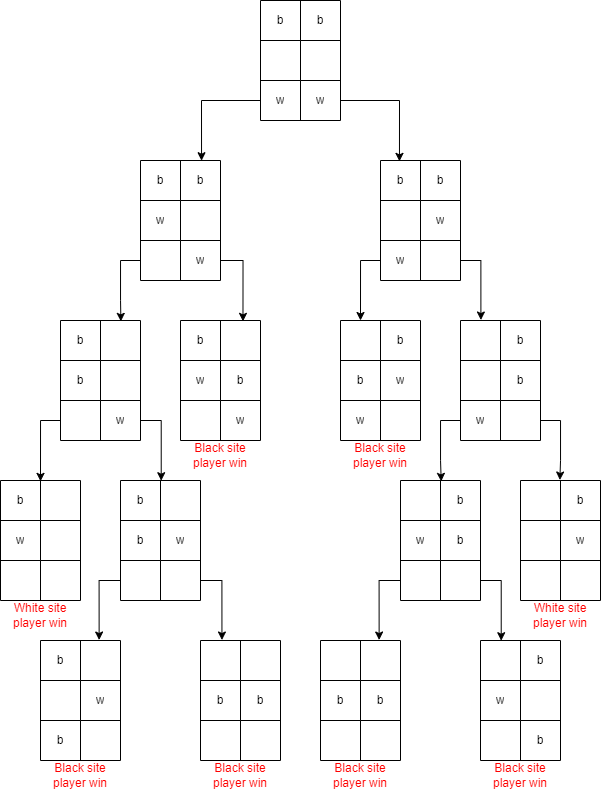
\includegraphics[width=\textwidth]{dependencies/pictures/Complete_Game_Tree.png}
        \caption{Complete game tree for simplified Hexapawn (w - white pawns, b - black pawns).}
        \label{fig:complete-game-tree-hexapawn}
    \end{figure}
    Last thing worth mentioning is the the fact that each game tree node consists not only from representation of chessboard, but also from evaluation value which has been assigned to this situation. However, this is a topic related directly to the functional aspect of the game tree which will be further discussed in section \ref{sec:min-max-algorithm}.

    \subsection{Min-max algorithm}\label{sec:min-max-algorithm}
    Even if game trees are crucial components while constructing AI, this component won't allow created instance for making decisions. To make those kind of operations \textbf{min-max tree} can be used. This structure i basically a game tree but every tree node consists also from evaluation value. Second difference between game tree and min-max tree is the fact that in second structure uses search algorithm called \textbf{min-max algorithm}. Before describing how min-max algorithm works it is important to explain how to evaluate each tree node. To calculate evaluation value for each nodes in the game tree evaluation functions are used. This type of function take as an input content of the tree node and return evaluation that needs to be assign to this node. More about evaluation functions in scope of this thesis can be found in section \ref{sec:game-tree-optimizations}.

    To explain how min-max algorithm works, generated game tree from \hyperref[fig:complete-game-tree-hexapawn]{fig. \ref*{fig:complete-game-tree-hexapawn}} will be used. Because generated tree present whole game (it is possible to see all outcomes), very simple evaluation function has been used. If given node resulted in white site player win, evaluation will be equal to $1$. Otherwise, evaluation will be equal to $-1$. The calculated values were assigned to proper nodes as it is presented on \hyperref[fig:min-max-tree-hexapawn]{fig. \ref*{fig:min-max-tree-hexapawn}}.
    \begin{figure}
        \centering
        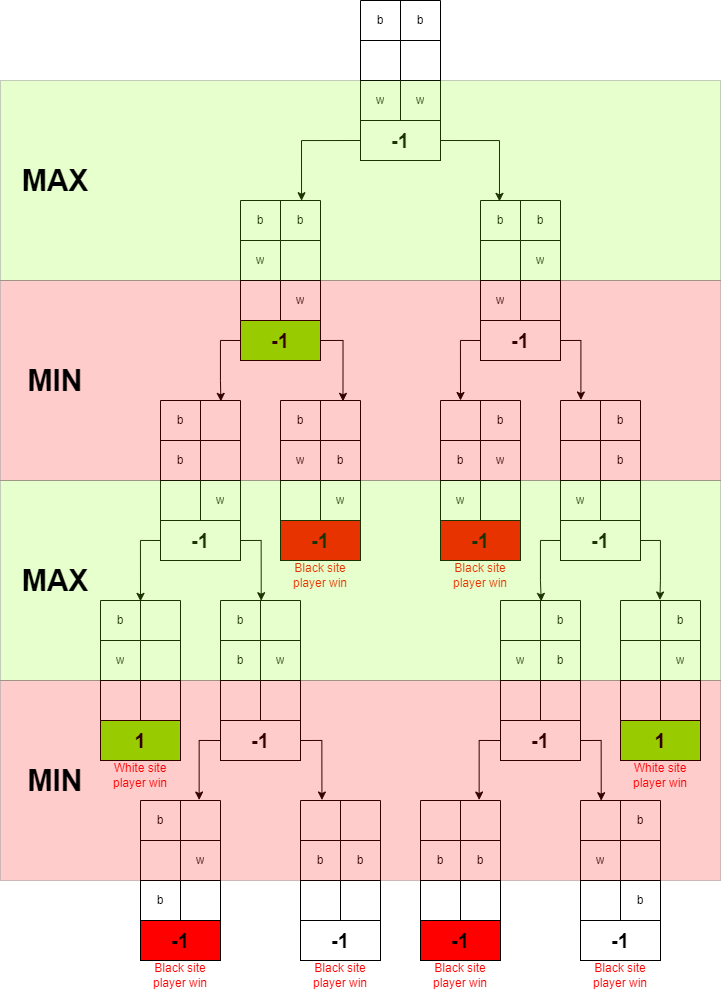
\includegraphics[width=0.8\textwidth]{dependencies/pictures/MinMax_Example.png}
        \caption{Min-max tree for simplified Hexapawn.}
        \label{fig:min-max-tree-hexapawn}
    \end{figure}

    As it can be seen on \hyperref[fig:min-max-tree-hexapawn]{fig. \ref*{fig:min-max-tree-hexapawn}}, it present also usage of min-max algorithm which will be now described.

    Structure analysis begins from is leafs. In the first iteration two nodes containing values $-1$ and $-1$ are compared. Because this layer represent opponent move, node with the lowest value got chosen (marked with red color). It happens because by definition, the opponent will make optimal moves, leading to a favorable situation for him. In the given situation, when both values are equal, first encountered value get chosen. After node comparison, chosen value is moved to node above for further comparisons. The same actions has been performed for rest nodes in this layer. After all nodes in last layer get compared, layer above needs to be analyze next. In case of this layer, comparing process is similar to te previous layer. Because analyzing layer represent AI move, among comparing nodes, the one with the highest value gets chosen (from both first nodes, value $1$ gets chosen and marked with green color). Similar like in last layer all chosen values are moved to layer above for further comparisons. By using this workflow, all root nodes evaluations needs to be calculated. Situation presented on \hyperref[fig:min-max-tree-hexapawn]{fig. \ref*{fig:min-max-tree-hexapawn}} shows that both root nodes have the same evaluation value so first encountered value get chosen \cite{bib:article-comparizon-of-search-algorithms}.

    \subsection{Game tree optimizations}\label{sec:game-tree-optimizations}
    Simplify version of game Hexapawn is simple enough it is possible to generate full game tree (resolve the game). Unfortunately, game that is a topic of this thesis is much more complex which means, resolving chess game is unreachable. Basing on average branching factor for chess game $b \approx 35$, and average game length $m \approx 70$, Victor Allis estimate complexity of the average game of chess to be $10^{123}$ \cite{bib:book-search-for-solutions-in-games}. That big complexity is potentially problematic because of big memorial and computational complexity of entire structure. Because of this complexity, a common practice is optimizing game tree size \cite{bib:article-optimal-on-game-trees}.

    The most commonly used optimization method is limiting depth of generating structure. In a lot of chess playing softwares, algorithm that generate game tree, do it until some constant value (most commonly this value is $3$) \cite{bib:internet-alphazero,bib:book-search-for-solutions-in-games,bib:article-optimal-on-game-trees}. This solution determine how many moves can be handled by created structure but prevents from solving the game. Usage of this optimization method force to use evaluation method because by analyzing only fragment of the game tree it is impossible to know all outcomes. There are multiple approaches to creating evaluation function. The simplest solution is to use heuristic equations \cite{bib:conference-heuristic-evaluation-chessai}. In this thesis evaluation will be handled by more complex solution, which is implemented and trained neural network instance. Used solution will be further described in section \ref{sec:neural-networks}. There are much more optimization methods that can be used, like $\alpha$-$\beta$ pruning, but in scope of this thesis, only game tree depth limitation has been used. 


    \section{Neural networks}\label{sec:neural-networks}
    As it was mentioned before, evaluation values that will be used in generated game tree, will be provided by neural network instance. While analyzing the problem it turned out that there are two types of neural network which can work with good effectiveness. As a scope of this thesis is to test which one of those two types of neural networks is more suitable for given problem of chess game. Two neural networks that will be described are Artificial Neural Network (ANN) and Convolutional Neural Network (CNN).

    \subsection{Artificial neural network}\label{sec:artificial-neural-network}
    To simplify further descriptions, it is better to start with ANN topic as it is the simplest version of any neural networks. Neural network is and mathematical structure model which uses basic processing elements (neurons) to perform some kind of operation on input data. An inspiration for this model is real-life neural systems. There are a lot of different types of neural networks but all of them consists of 2 main components: neuron and weight \cite{bib:internet-neural-network-and-deep-learning}. To avoid misunderstanding, in the further part of this thesis, both ,,artificial neural network'' and ,,neural network'' will relate to the same type of neural network. Artificial neural network in its most basic form can consists of following elements:
    \begin{description}
        \item[Weight] represent the connection between neurons. Each weight have also value assign to it which represent how strong particular connection is. Weights values are first of parameters that are modified in learning process. Learning process for ANN will be further described in this section (\ref{sec:learning-process-for-nn-instance}).
        \item[Neuron] is the most basic element of neural network. It is element performing mathematical operation on input data and as an output it return just single value. Output value of neuron $k$ in layer $m$ ($n_k^{(m)}$) can be calculated using following equation:
        \begin{equation}\label{eq:ann-neuron-value}
            n_k^{(m)} = f\left(b_i + \sum_{i = 0}^{l} w_{m-1, i} n_i^{(m-1)}\right),
        \end{equation}
        where:
        \begin{itemize}[label=]
            \item $n_i^{(m-1)}$ -- output value of neuron $i$ in layer $(m-1)$, $w_{m-1, i}$ -- weight value from neuron $i$ in layer $(m-1)$, $b_i$ -- value of bias $i$, $l$ -- number of neurons in layer $(m-1)$, $f$ -- activation function.
        \end{itemize}
        As it can be seen in equation \eqref{eq:ann-neuron-value} activation function was used. In this thesis, for artificial neural network, sigmoid function has been used ($a=\frac{1}{1 + e^{-n}}$). This activation function squash input value in range $(0, 1)$ but another, often used range o this function is $(-1, 1)$ \cite{bib:internet-sigmoid-function}. In case of this thesis, second range has been used.
        \item[Layer] works as and organization unit for neurons which define in which order, those neurons will be processed. Usually, artificial neural network consists of 3 types of layer \cite{bib:book-make-own-neural-network}:
        \begin{itemize}
            \item Input layer -- represent group of neurons containing input data. Neurons in this layer do not have weights and their value are not passed through activation function.
            \item Hidden layer -- represent group of neurons which are located between first and last layer of the network. Number of hidden layers and number of their neurons are not strictly defined and often it needs to be experimented with, to find the best setup for given problem.
            \item Output layer -- represent group of neurons located at the end of the network which is also network answer for given problem.
        \end{itemize}
        \item[Bias] is a additional neuron in each layer which is used for output regulations. This neuron also have weight value, that is why this weight value can be skipped in output calculations. Value of the bias is added to final sum of neuron values and their weights as it has been shown in equation \ref{eq:ann-neuron-value}. Value of the bias is the second modifiable parameters, changed in learning process.
    \end{description}
    For better understanding of neural network structure, on \hyperref[fig:ann-example]{fig. \ref*{fig:ann-example}} has been shown simple example of this kind of network. As it can be seen, this network consists of 3 layers (1 input layer, 1 hidden layer and 1 output layer) and value from input layer gets propagated through all other layers.
    \begin{figure}
        \centering
        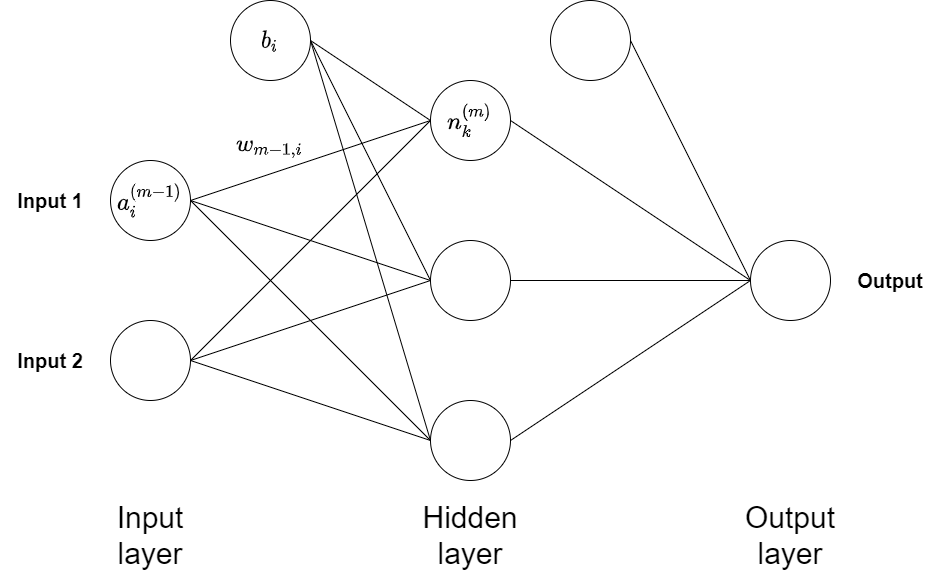
\includegraphics[width=0.8\textwidth]{dependencies/pictures/NN_example.png}
        \caption{Artificial neural network example.}
        \label{fig:ann-example}
    \end{figure}
    Process shown of \hyperref[fig:ann-example]{fig. \ref*{fig:ann-example}} is called \textbf{feed forward algorithm} and constitute whole process of resolving problems in neural networks. Feed forward process begins from loading input data into input layer. Then, by using equation presented in \ref{eq:ann-neuron-value}, those values are propagated through all hidden layers (if their exist) and lastly, final answer can be seen in output layer \cite{bib:book-make-own-neural-network,bib:article-application-of-feedforward-for-grade-estimation,bib:internet-neural-network-and-deep-learning}. It was decided to use this type of neural network, for chess game problem, because it is the most basic type of neural network so it will be very good comparison point for other used models.

    \subsection{Convolutional neural network}
    As it was mentioned before, scope of this thesis is to compare two neural network models and decide which one performs better in case of chess game problem. Second type of neural network that will be used for this task is Convolutional Neural Network. Why this type of network? Convolutional neural networks (CNN) act as pattern detecting algorithm. The most common usages of this model are: cancer detection, picture classifications, face detection, recognizing hand-written digits etc. \cite{bib:internet-real-world-applications-of-cnn}. Because of this fantastic performance while detecting patterns, this type of neural network can also be able to detect patterns on chessboard which will result in good evaluation of chessboard situations. To see how good this model will perform with this problem, it will be compared with the most basic neural network described in section \ref{sec:artificial-neural-network}.

    Now, when structure of artificial neural network has been described, it is possible to explain CNN structure. Convolutional neural network can consists of 4 types of layer:
    \begin{description}
        \item[Fully-connected/Dense layer] is the same type of layer that exist in artificial neural network. This layer has been described in \ref{sec:artificial-neural-network}. In case of CNN, dense layer are used as an input an output layers.
        \item[Convolutional layer] is the most important component of this network, which is responsible for detecting patterns. In contrast to dense layer, where an input is a vector of values, in convolutional layer input is an matrix of values. On this input matrix is performed \textbf{Convolution} operation and acquired matrix is passed to next layer. Convolutional layer will be further described in section \ref{sec:convolutional-layer}.
        \item[Pooling layer] is a type of layer which reduce size of input matrix. This layer is used to reduce time and memory consumption and to make sure that only ,,important'' sections of the input matrix will be used for further computations. More information about this layer can be found in section \ref{sec:pooling-layer}.
        \item[Activation layer] is a type of layer which apply activation function on the input matrix. There are a lot of possible choices for activation function, like sigmoid function (see section \ref{sec:artificial-neural-network}), but in scope of this thesis, ReLU (Rectified Linear Unit) activation function has been used. ReLU function can be described by equation $f(x) = max(0, x)$. To simplify, all negative numbers are changed to $0$ and all positive numbers stays unchanged \cite{bib:internet-relu-function}.
    \end{description}
    Basic structure of convolutional neural network is presented on \hyperref[fig:cnn-example]{fig. \ref*{fig:cnn-example}}
    \begin{figure}
        \centering
        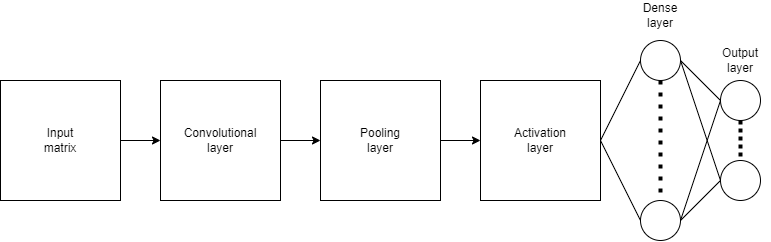
\includegraphics[width=\textwidth]{dependencies/pictures/CNN_example.png}
        \caption{Convolutional neural network example.}
        \label{fig:cnn-example}
    \end{figure}

    \subsubsection*{Convolutional layer}\label{sec:convolutional-layer}
    As it was mentioned before, convolutional layer is capable of detecting patterns (features) such as edges on given input picture. This process can be done with use of filters (also known as kernels). Kernels are small matrices containing numbers which also are modifiable parameters used in learning process. Each  convolution layer consists of some number of kernels from which each of them is used to detect some kind of pattern. For example, to recognize hand-written $1$, two kernels can be used. First for detecting diagonal line and second one to detect straight line.

    To check if given pattern exist in input data, each convolution layer perform \textbf{Cross-correlation} operation on input data and all kernels. Cross-correlation can be performed by ,,sliding'' given kernel matrix over input data and computing \textbf{Frobenius inner product} (summing calculated element-wise multiplication products) \cite{bib:book-frobenius-inner-product} for all intersections. That calculated values creates output matrix of the cross-correlation operation. Mathematical equation for cross correlation can be written as follows:
    \begin{equation}
        G[i, j] = \sum_{u = 0}^{l} \sum_{v = 0}^{k} h[u, v] F[i+u. j+v],
    \end{equation}
    \begin{equation}
        G = h \bigotimes F,
    \end{equation}
    where:
    \begin{itemize}[label=]
        \item $G[i, j]$ -- output matrix value of indexes $i$ and $j$, $l$ -- size of the input matrix, $k$ -- size of the kernel, $h$ -- kernel, $F$ -- input matrix \cite{bib:article-cross-correlation}.
    \end{itemize}
    Example of cross-correlation operation can be seen on \hyperref[fig:cross-correlation-example]{fig. \ref*{fig:cross-correlation-example}}.
    \begin{figure}
        \centering
        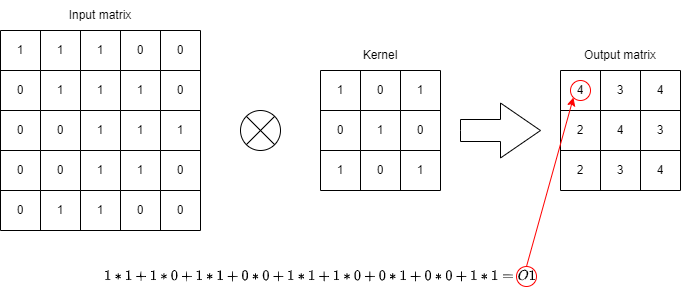
\includegraphics[width=\textwidth]{dependencies/pictures/Cross-correlation_example.png}
        \caption{Cross-correlation example.}
        \label{fig:cross-correlation-example}
    \end{figure}
    Important thing to mention is the fact that cross-correlation operation can be performed with different \textbf{stride} (size of the step with which kernel is sliding over input matrix). The most common stride to use is $1$ but it can be changed. In case of this thesis, all cross-correlation operations are performed with stride of $1$. It is possible to calculate size of cross-correlation output matrix by using equation:
    \begin{equation}
        n_{out} = floor((l - k) / s) + 1,
    \end{equation}
    where:
    \begin{itemize}[label=]
        \item $n_{out}$ -- size of output matrix, $l$ -- size of the input matrix, $k$ -- size of the kernel, $s$ -- stride.
    \end{itemize}

    In each convolutional layer first think that is performed on input data is a cross-correlation between input matrix and all the kernels that the layer consists of. Important thing to mention is the fact that the output of the convolutional layer can be different. Number of matrices produced by layer is determine by number of kernels inside that layer. After performing cross-correlation operation, to each output matrix is added bias matrix \cite{bib:internet-aa-cnn-lecture}. In conclusion, output of convolutional layer with one kernel can be described by equation:
    \begin{equation}
        Conv_{out} = h \bigotimes F + B,
    \end{equation}
    where:
    \begin{itemize}[label=]
        \item $Conv_{out}$ -- convolutional layer output matrix, $h$ -- kernel, $F$ -- input matrix, $B$ -- bias matrix.
    \end{itemize}

    \subsubsection*{Pooling layer}\label{sec:pooling-layer}
    Pooling layer is the second distinctive element of convolutional neural network. As it was mentioned before, main purpure of pooling layer is to reduce size of the matrix that is used for calculations. There are a lot of possible functions that can be performed in this layer but two the most common are \textbf{Max Pooling} and \textbf{Average Pooling} \cite{bib:book-pooling-methods}. In case of this thesis, Max Pooling method has been used. 

    Max pooling method is also used to highlight the most important parts of the feature map. This operation works in the similar way to cross-correlation operation. Each pooling layer consists of window of the specific size which slide over input matrix, with specific stride (similar like in cross-correlation operation). While sliding over input matrix, algorithm pick maximal value and pass it into output matrix. Max pooling example can be seen on \hyperref[fig:max-pooling-example]{fig. \ref*{fig:max-pooling-example}}
    \begin{figure}
        \centering
        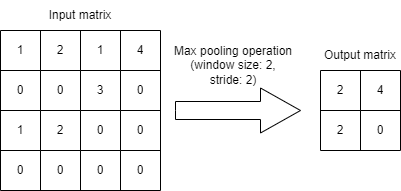
\includegraphics[width=\textwidth]{dependencies/pictures/Max_Pooling_example.png}
        \caption{Max pooling example.}
        \label{fig:max-pooling-example}
    \end{figure}

    \subsection{Learning process for neural network instance}\label{sec:learning-process-for-nn-instance}
    After describing two types of neural network that will be used in following thesis, last thing that needs to be explained is learning process. This process looks similar in both neural networks (ANN and CNN) so it will bee described as one. When neural network is created, values of all weights and biases are set randomly and that will result in network answers also being random \cite{bib:article-how-neural-network-learn}. To make network answers more sensible it needs to be ,,taught'' how to approach the problem. Method of machine learning that will be used to improve neural network answers is called \textbf{supervised learning}. This type of learning method is based on examples and target output. Dataset that is used for training needs to have input data and target data to calculate how ,,bad'' was model answer \cite{bib:book-statistical-learning}. Learning process consists in periodic algorithm which will result in updating values of weights and biases. This process begins with splitting data set into two sets (training set and test set). Next, each example of training set need to be inputted into model and output needs to be read. When model output will be acquired it needs to be compared with target data for given example. One of the methods of performing this comparison is to calculate \textbf{loss function}. This is place is the first one in which learning process for ANN and CNN is slightly different. For both models loss function will be calculated, but formula for calculating this function will be different in each type of network. Loss function for artificial neural network will be calculated using formula:
    \begin{equation}
        \lambda_{ANN} = t - ANN_{out},
    \end{equation}
    where:
    \begin{itemize}[label=]
        \item $\lambda_{ANN}$ -- value of loss function for artificial neural network, $t$ -- target value for given example, $ANN_{out}$ -- output of the model.
    \end{itemize}
    Loss function for convolutional neural network will be calculated using formula:
    \begin{equation}
        \lambda_{CNN} = -\sum t \log CNN_{out},
    \end{equation}
    where:
    \begin{itemize}[label=]
        \item $\lambda_{CNN}$ -- value of loss function for convolutional neural network, $t$ -- target value for given example, $CNN_{out}$ -- output of the model.
    \end{itemize}
    By calculating loss functions for both models, it is possible to check how incompatible models answers are from desirable output. 

    Unfortunately, knowing how bad specific model performs in given task, won't result in making it better. To improve performance of given model, \textbf{Backpropagation algorithm} can be used \cite{bib:book-make-own-neural-network,bib:internet-convolutions-and-backpropagation}. Backpropagation algorithm is the most important component in whole learning process because this methodology allows for improving how model perform. Main idea of this algorithm is backward propagation of computed error (loss function), which is based on calculating \textbf{gradient} value for given loss function ($\nabla f$). Result of this operation is the set of values which shows how values of output layer should change to decrease loss function. Unfortunately, there is no possibility to change neurons values directly. There is possibility to impact neuron value by modifying following components: 
    \begin{itemize}
        \item values of input weights,
        \item value of biases,
        \item values of neurons in previous layer.
    \end{itemize}
    The same methodology can be applied to all layers in the network. Last important thing, worth mentioning, is the fact that learning process for both ANN and CNN looks the same but equations, used for calculating gradient are different for each network type.

    In conclusion, learning process of neural network model can be described by 5 steps:
    \begin{enumerate}
        \item Load training data into model,
        \item Using feedforward algorithm obtain output of the model,
        \item Calculate loss function for given example,
        \item Using backpropagation algorithm, calculate gradient values for all weights and biases,
        \item Update values of all weights and biases.
    \end{enumerate}
    After processing all examples from training set, test set is used to check model accuracy. If accuracy is to low, it is necessary to repeat training process. This sequence of action can be repeated until obtained accuracy will be acceptable (potentially, global minimum of the loss function will be achieved) \cite{bib:internet-aa-cnn-lecture,bib:book-make-own-neural-network}. To improve, obtained results and to increase probability of finding global minimum of the loss function, there is 1 modification of backpropagation algorithm that will be used in scope of this thesis. There is parameter called \textbf{learning rate} \cite{bib:internet-learning-rate}. This is value which define how big changes will be applied to weights and biases. Because final goal of the backpropagation algorithm is finding global minimum of the loss function, if the changes will be to big, it can result in constant passing the proper minimum value. Usage of proper learning rate value reduce probability of it happening.

    \section{Other approaches to the problem}\label{sec:other-approaches-to-problem}
    After describing problem approach that will be used in scope of this thesis, it is important to mention what other solutions to the Chess AI problem can be found. First approach is very similar to described solution because it uses all mentioned components except of neural network instance. This solution assumes usage of complex mathematical equations to evaluate chessboard situation. This type of approach is caller \textbf{heuristic approach} \cite{bib:article-computer-chess-move-ordering,bib:internet-step-by-step-chess-ai}. The main problem of heuristic approach is the fact that this solution is very time consuming and require big knowledge of chess game to implement correctly. Another disadvantage of this approach is the fact that it is very linear solution and it is hard to implement some unpredictability which can result in small effectivity against more advanced chess players.

    Second possible approach looks much more promising but it is also much harder to implement. This approach assumes usage of self-improving neural network. Mentioned before AlphaZero software uses this exact method for playing \cite{bib:internet-alphazero}. Basic idea behind this approach is to create some kind of algorithm which will be building and modifying neural network structure while playing with real opponent. This method is very popular and very efficient in game theory because it can result in creating ,,unbeatable'' AI. Main advantage of this solution is the fact that the more games will be played by AI instance, the smartest it gets \cite{bib:article-self-improving-nn}. Usage of this method can result in very interesting results but it is also very hard to implement. Another problem regarding this solution is time consumption and quality of ,,training resources''. If created AI will play with the best players, it will learn a lot but in the other case it can stop improving.

% References to 
% book \cite{bib:book},
% scientific papers in journals \cite{bib:article},
% conference papers \cite{bib:conference},
% and web pages \cite{bib:internet}.

% Equations should be numbered:
% \begin{align}
% y = \frac{\partial x}{\partial t}
% \end{align}

%\chapter{[Problem analysis]}
%
%\begin{itemize}
%\item problem analysis, problem statement
%\item state of the art, literature research (all sources in the thesis have to be referenced, eg journal article \cite{bib:article} book \cite{bib:book}, conference paper \cite{bib:conference}, internet source \cite{bib:internet})
%\item description of known solutions, algorithms
%\item location of the thesis in scientific domain
%\item The title of this chapter is similar to the title of the thesis.
%\end{itemize}
 

% TODO


\chapter{Subject of the thesis}
Building Chess AI is very difficult and time consuming process if it is require to achieve good effectiveness. In scope of this thesis an approach has been used that includes the following components:
\begin{itemize}
	\item game tree as an decision making structure,
	\item min-max algorithm as an search algorithm,
	\item game tree depth limit as an optimization method,
	\item artificial neural network as an first evacuation function,
	\item convolutional neural network as an second evaluation function.
\end{itemize}

\section{Decision making system - implementation}
Starting game tree structure is generated at the beginning of the program using recursive method. At the beginning of the program, there is option to choose game tree depth limit. This configuration specify how many moves needs to be included in game tree structure. When last layer of the structure will be achieved, game tree will be destroyed and regenerated with the same depth. As it was described in section \ref{sec:game-tree-optimizations}, it is impossible to generate full game tree of chess, so that is why game tree depth limitation has been used. The most commonly used game tree depth limit is $3$. It is possible to specify different value of this parameter but it is important to keep in mind that it will impact time needed to make decision. Example structure of game tree used in the the project can be seen on \hyperref[fig:game-tree-fragment]{fig.  \ref*{fig:game-tree-fragment}}.
\begin{figure}
	\centering
	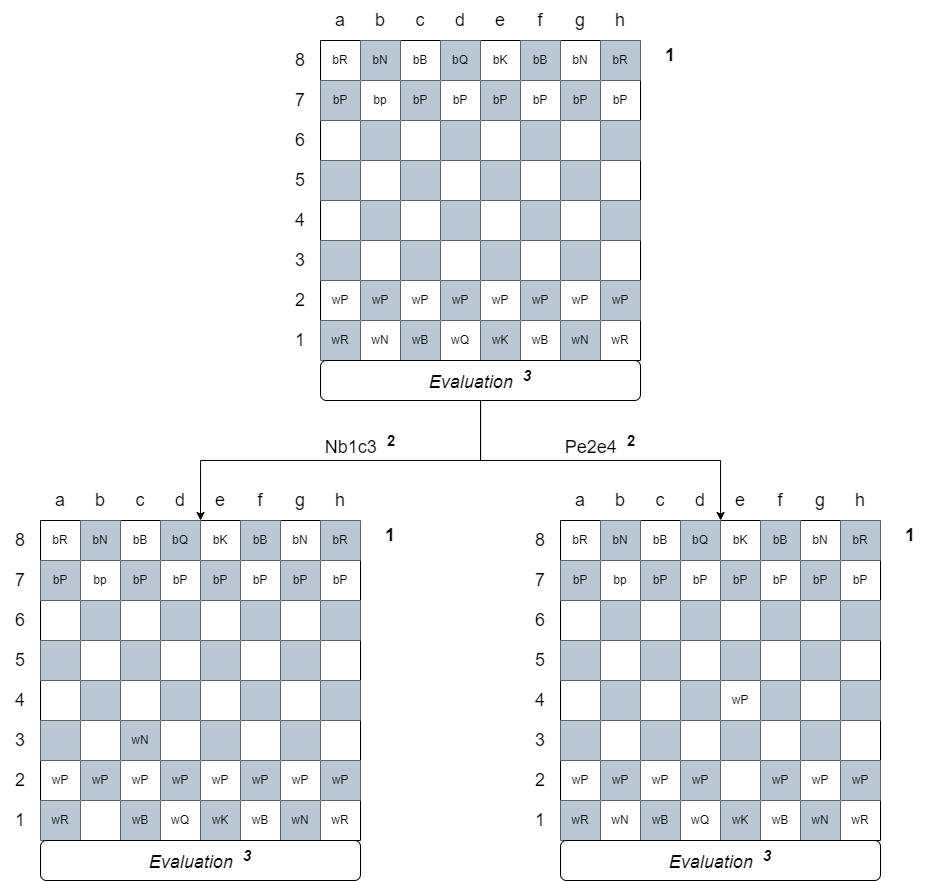
\includegraphics[width=\textwidth]{dependencies/pictures/Game_Tree_Fragment_Example.png}
	\caption{Game tree fragment example (1 - chess board representation, 2 - move command, 3 - evaluation value).}
	\label{fig:game-tree-fragment}
\end{figure}

Created game tree is used as an input to the min-max search algorithm. Detail explanation of this algorithm can be found in section \ref{sec:min-max-algorithm}. There are 2 main assumptions that needs to be explain while describing usage of min-max algorithm in scope of this thesis. If game take place in scenario ,,player vs AI'', human player always is assign to white site of the board which also result in making first move. If game scenario is set to be ,,AI vs AI'', each of the instances gets assign randomly to one of the site. Sequence in which min-max algorithm work can be specified as follows:
\begin{enumerate}
	\item Find the most beneficial sequence of moves in generated game tree.
	\item Get chessboard situation after opponents move.
	\item If gathered node is not one of game tree nodes, go back to point 1. Otherwise, regenerate game tree and go back to point 1.
\end{enumerate}
Important thing to mentioned is the fact that in scope of this thesis there are no optimization method used for min-max algorithm. It can result in increasing time of making decisions while playing. It was decided to use min-max tree structure because it is core element of a lot of other chess playing AI and it it the mos beneficial solution. 

\section{Evaluation system - implementation}\label{sec:evaluation-system-implementation}
To make all experiments more accurate, it ha been decided to implement very basic models of ANN and CNN. To increase accuracy even more, both instances were coded from scratch and trained on the same datasets. Using neural network model as an evaluation method is not a new approach but usage of CNN and ANN, on the other hand is, because the most often used models are genetic algorithm based one. It is hard to predict how effective this approach would be, before analyzing tests results, but it can be very interesting how it perform. 

Before further discursion it is necessary to describe how chessboard is represented in the final program. There are $3$ methods that chess pieces are stored: number type, string type and object type. All of those types are shown in \hyperref[tab:chess-pieces-types]{tab. \ref*{tab:chess-pieces-types}} (object type will be skipped in the table).
\begin{table}
	\centering
	\caption{The list of chess pieces types.}
	\label{tab:chess-pieces-types}
	\begin{tabular}{ccc}
	\toprule
		\textbf{symbol} & \textbf{number value} & \textbf{string value}\\
		\hline
			\WhiteKingOnWhite \BlackKingOnWhite & 7 / -7 & wK / bK\\
		\hline
			\WhiteQueenOnWhite \BlackQueenOnWhite & 5 / -5 & wQ / bQ\\
		\hline
			\WhiteBishopOnWhite \BlackBishopOnWhite & 4 / -4 & wB / bB\\
		\hline
			\WhiteKnightOnWhite \BlackKnightOnWhite & 3 / -3 & wN / bN\\
		\hline
			\WhiteRookOnWhite \BlackRookOnWhite & 2 / -2 & wR / bR\\
		\hline
			\WhitePawnOnWhite \BlackPawnOnWhite & 1 / -1 & wP / bP\\
	\end{tabular}
\end{table}
Data structure containing numerical values representing chess pieces will be used as an input in both instances of created neural networks.

\subsection{Artificial neural network - architecture}\label{sec:ann-architecture}
As it was mentioned before, each of neural network instances was implemented from scratch to make experiments more reliable. When creating artificial neural network instance, there are two main aspects that needs to be specified. First and the most crucial topic is to design architecture of the network. Because problem that needs to be solved is evaluating chessboard situation, created network needs to take $64$ values as an input (chessboard have dimension of $8 \times 8$) and needs to return one value which will be assigned as an evaluation value to the specific chessboard situation. To keep created model as simple as possible, it has been decided to include only two hidden layers with $64$ neurons each. When structure of the network has been created, there is one last important configuration to establish. As it was mentioned in section \ref{sec:learning-process-for-nn-instance}, every instance of neural network needs to have learning rate parameter specified. During training process, it was established that learning rate value for artificial neural network should be equal to $0.001$. This value resulted in the most efficient training process for this model. It is possible that ANN evaluation function will not provide spectacular results for given problem but it is important to remember that it has been used as an basic point of comparison for second evaluation. This method allows to decide if usage of CNN, for evaluating chessboard situations, is an justified or beneficial solution to the problem.

\subsection{Convolutional neural network - architecture}\label{sec:cnn-architecture}
While planing structure for convolutional neural network, the main goal was to keep structure of the model simple. This decision has been made because if basic structure of CNN model won't perform better than basic structure of ANN, it is a proof that given solution is bad. Second reason for keeping model structure simple is less time consuming training process for both models. There are two elements in convolutional neural network configuration that are similar to the first used model. The best value for learning rate parameter is equal to $0.001$ and sizes of input and output layers are also the same like in artificial neural network. It has been decided that CNN model will consists of two convolutional layers, with 13 and 10 kernels respectively, two pooling layers, two activation layers and one fully connected layer. Full structure of the used CNN can be found on \hyperref[fig:cnn-structure]{fig. \ref*{fig:cnn-structure}}.
\begin{figure}
	\centering
	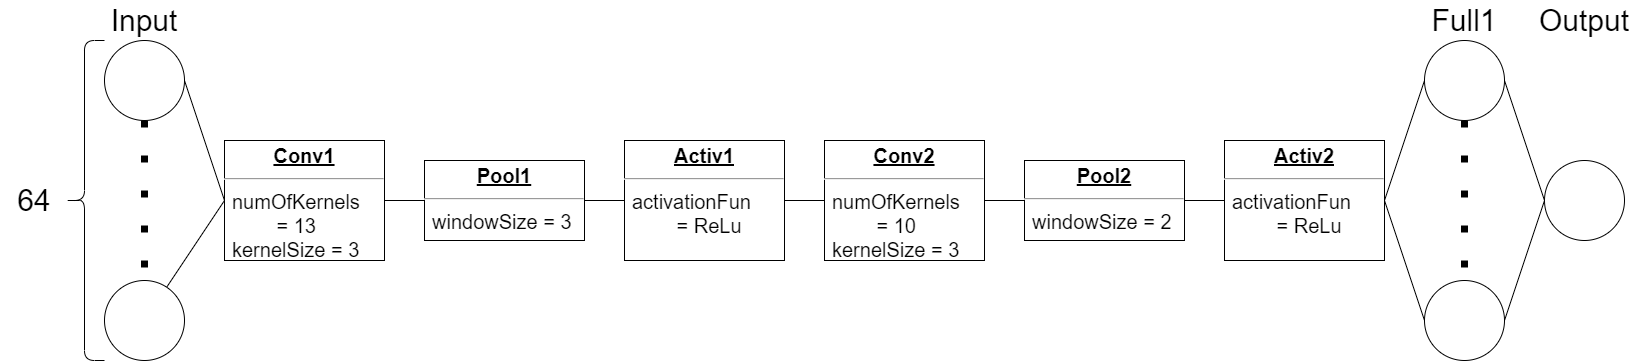
\includegraphics[width=\textwidth]{dependencies/pictures/CNN_Structure.png}
	\caption{Structure of the implemented CNN.}
	\label{fig:cnn-structure}
\end{figure}
In the contrary to ANN hidden layers, which number of neurons are not backed by any theoretical aspects, convolutional layers was design based on chess game theory. According to publications about chess there are $13$ the best openings which give player the most benefits. This is why first convolutiona layer consists of $13$ kernels. Second convolutional layer consists of $10$ kernels because this is the number of the most commonly used, beneficial chessboard arrangements \cite{bib:book-mastering-chess-logic,bib:book-chess-bible,bib:book-bobby-fisher-teaches-chess}. The assumption is that both convolutional layers will be responsible for detecting mentioned chessboard arrangements.

\section{Used tools}
In the scope this thesis, all components of the final project has been implemented from scratch using C++17 language. As an IDE Visual Studio Code (VSCode) has been chosen. To build and prepare project for compilation Premake software has been used. This thesis has been written using \LaTeX language and VSCode IDE. For creating all diagrams used in this thesis, Draw.io online software has been used. In the creative process of this project, the sources included in the bibliography and following documentations were used: \cite{bib:internet-c++-doc,bib:internet-latex-doc,bib:internet-vscode-doc,bib:internet-premake-doc}.

% tekst

% \section{[Section title]}

% \section{[Subsection title]}

% Each figure in the document should be referred to at least once (fig. \ref{fig:2}).

% \begin{figure}
% \centering
% \begin{tikzpicture}
% \begin{axis}[
%     y tick label style={
%         /pgf/number format/.cd,
%             fixed,   % po zakomentowaniu os rzednych jest indeksowana wykladniczo
%             fixed zerofill, % 1.0 zamiast 1
%             precision=1,
%         /tikz/.cd
%     },
%     x tick label style={
%         /pgf/number format/.cd,
%             fixed,
%             fixed zerofill,
%             precision=2,
%         /tikz/.cd
%     }
% ]
% \addplot [domain=0.0:0.1] {rnd};
% \end{axis} 
% \end{tikzpicture}
% \caption{Figure caption.} % Figure caption is BELOW the figure!
% \label{fig:2}
% \end{figure}

% Each table in the document should be referred to at least once (Tab. \ref{tab:results}).

% \begin{table}
% \centering
% \caption{A caption of a table is ABOVE it.}
% \label{tab:results}
% \begin{tabular}{rrrrrrrr}
% \toprule
% 	         &                                     \multicolumn{7}{c}{method}                                      \\
% 	         \cmidrule{2-8}
% 	         &         &         &        \multicolumn{3}{c}{alg. 3}        & \multicolumn{2}{c}{alg. 4, $\gamma = 2$} \\
% 	         \cmidrule(r){4-6}\cmidrule(r){7-8}
% 	$\zeta$ &     alg. 1 &   alg. 2 & $\alpha= 1.5$ & $\alpha= 2$ & $\alpha= 3$ &   $\beta = 0.1$  &   $\beta = -0.1$ \\
% \midrule
% 	       0 &  8.3250 & 1.45305 &       7.5791 &    14.8517 &    20.0028 & 1.16396 &                       1.1365 \\
% 	       5 &  0.6111 & 2.27126 &       6.9952 &    13.8560 &    18.6064 & 1.18659 &                       1.1630 \\
% 	      10 & 11.6126 & 2.69218 &       6.2520 &    12.5202 &    16.8278 & 1.23180 &                       1.2045 \\
% 	      15 &  0.5665 & 2.95046 &       5.7753 &    11.4588 &    15.4837 & 1.25131 &                       1.2614 \\
% 	      20 & 15.8728 & 3.07225 &       5.3071 &    10.3935 &    13.8738 & 1.25307 &                       1.2217 \\
% 	      25 &  0.9791 & 3.19034 &       5.4575 &     9.9533 &    13.0721 & 1.27104 &                       1.2640 \\
% 	      30 &  2.0228 & 3.27474 &       5.7461 &     9.7164 &    12.2637 & 1.33404 &                       1.3209 \\
% 	      35 & 13.4210 & 3.36086 &       6.6735 &    10.0442 &    12.0270 & 1.35385 &                       1.3059 \\
% 	      40 & 13.2226 & 3.36420 &       7.7248 &    10.4495 &    12.0379 & 1.34919 &                       1.2768 \\
% 	      45 & 12.8445 & 3.47436 &       8.5539 &    10.8552 &    12.2773 & 1.42303 &                       1.4362 \\
% 	      50 & 12.9245 & 3.58228 &       9.2702 &    11.2183 &    12.3990 & 1.40922 &                       1.3724 \\
% \bottomrule
% \end{tabular}
% \end{table}  


%\chapter{[Subject of the thesis]}
%
%\begin{itemize}
%\item solution to the problem proposed by the author of the thesis
%\item theoretical analysis of proposed solutions
%\item rationale of applied methods, algorithms, and tools
%\end{itemize} 

% TODO
\chapter{Experiments}\label{sec:experiments}
The first important thing that needs to be discussed before describing experiments is machine on which experiments have been performed. Experimental machines properties looks as follows:
\begin{itemize}
    \item Operating system: Windows 10 Professional,
    \item Processor: Intel(R) Core i5-11400F
    \begin{itemize}
        \item 11th generation,
        \item 2.60GHz
    \end{itemize}
    \item RAM: 16 GB DDR4,
    \item Graphical card: NVIDIA GeForce GTX 970,
    \item Hard drive: 500 GB SSD.
\end{itemize}
Those parameter can be changed but it is important to remember that used game tree structure is very memory consuming and neural network training require a lot of computation power. It is recommended to use specified parameters of higher. Last important thing to mention is the fact that result application has been created for Windows operating system only and wasn't tested on other operating systems.

\section{Methodology}\label{sec:methodology}
Performed tests was divided into three sets of tests:
\begin{description}
    \item[Neural network training] this set of tets was based on training created neural network instances. It allows for finding the most optimal values of learning rate parameter. After that, AI instances were tested for number of iterations (epochs) require to get the best accuracy and number of data require for training. More information about datasets used for training can be found in section \ref{sec:data-sets}.
    \item[Manual testing] this set of tests relied on playing against AI instances in ,,player vs AI'' scenario. This set of tests covered test case in which player play against trained and untrained AI instance. Important thing to mention is the fact that this set of tests required both neural networks to be trained on the same size of data set. Otherwise, experiment would be unreliable.
    \item[Automated testing] this set of test was performed in ,,AI vs AI'' scenario. The main goal of this testing was to perform small ,,tournament'' to check which AI instance performs better. Similarly to te manual testing, this set of test has been performed with trained and untrained neural networks. Both neural networks was trained with the same data set.
\end{description}

\subsection{Chess application}
To perform mentioned tests, it was necessary to have application that allows for chess game. Application has been created and while starting it it is possible to specify which execution scenario needs to be performed. Because application uses command line interface, execution configuration is passed by input parameters. By specifying \texttt{--exScenario} parameter, application can be started in one of 3 modes:
\begin{itemize}
    \item parameter value: \texttt{0} - application will start in mode ,,player vs player'',
    \item parameter value: \texttt{1} - application will start in mode ,,player vs AI'',
    \item parameter value: \texttt{2} - application will start in mode ,,AI vs AI''.
\end{itemize}
Default value of this parameter is set on \texttt{0}. If \texttt{--exScenario} parameter will have value \texttt{1} or \texttt{2} application will ask for game tree limit to be specified (\hyperref[fig:setting-game-tree-depth]{fig. \ref*{fig:setting-game-tree-depth}}). If user won't specify this parameter, its value will be set on $3$.
\begin{figure}
    \centering
    \VerbatimInput{dependencies/documents/Setting_Game_Tree_Depth.txt}
    \caption{Menu allowing for specify game tree depth.}
    \label{fig:setting-game-tree-depth}
\end{figure}

\subsubsection{Chess application - manual control}
Choosing proper execution mode for the application, have impact on method of controlling application. If \texttt{--exScenario} parameter will have value \texttt{0} or \texttt{1}, application will show proper menu presented on \hyperref[fig:application-main-page]{fig. \ref*{fig:application-main-page}}
\begin{figure}
    \centering
    \VerbatimInput{dependencies/documents/Application_Main_Page.txt}
    \caption{Application main page.}
    \label{fig:application-main-page}
\end{figure}
Application main menu allows user to choose one of three options:
\begin{description}
    \item[New game] (command \texttt{N} / \texttt{n}) which reset all environment configurations and start new, fresh game. Choosing this option allows to set new game tree depth.
    \item[Move] (command \texttt{M} / \texttt{m}) which allows user to perform move. Choosing this option allows to select option \texttt{?} which print out information about legal moves syntax.
    \item[Quit] (command \texttt{Q} / \texttt{q}) which close application.
\end{description}
Last thing worth mentioning is move command syntax. For move command to be accepted by the system, it is require to specify horizontal coordinate (a \dots h) first and vertical coordinate (1 \dots 8) second.
\begin{itemize}
    \item \textbf{Syntax: <piece-id><starting-position><ending-position>}
    \item \begin{itemize}[label={}]
        \item where:
        \begin{itemize}[label={}] 
            \item piece-id := \{K -- king, Q -- queen, B -- bishop, N -- knight, R -- rook, P -- pawn\}
            \item starting-position / ending-position := \{a1\dots h8\}
        \end{itemize} 
        \item description: Performs traditional move. Traditional capturing is also handled by this command.
        \item example: Nb8a6.   
    \end{itemize}
    \item \textbf{Syntax: 0-0}
        \begin{itemize}[label={}]
            \item description: Performs short castling. 
        \end{itemize}
    \item \textbf{Syntax: 0-0-0}
        \begin{itemize}[label={}]
            \item description: Performs long castling. 
        \end{itemize}
    \item \textbf{Syntax: \texttt{P<starting-position>-><piece-id>}}
        \begin{itemize}[label={}]
            \item where:
            \begin{itemize}[label={}]
                \item starting-position := \{a1\dots h8\}
                \item piece-id := \{K -- king, Q -- queen, B -- bishop, N -- knight, R -- rook, P -- pawn\} 
            \end{itemize}
            \item description: Promote pawn to chosen piece.
            \item example: Pb7->Q. 
        \end{itemize}
    \item \textbf{Syntax: \texttt{P<starting-position>x<first-coordinate-ending-position>}}
        \begin{itemize}[label={}]
            \item where:
            \begin{itemize}[label={}]
                \item starting-position := \{a1\dots h8\}
                \item first-coordinate-ending-position := \{a\dots h\} 
            \end{itemize}
            \item describing: Performs en-passant manoeuver.
            \item example: Pc4xd.
        \end{itemize}
\end{itemize}

\subsection{Chess application - automated control}
If \texttt{--exScenario} parameter will have value \texttt{2}, application will also show chessboard abd capture lists but control will be limited. After each turn, user will be able to continue game or stop it and exit application. This option was implemented to provide infinite games in which both AI instances play on the same level.

\section{Data sets}\label{sec:data-sets}
To train created neural network instances, PGN files were used. Those are text file that contains records of chess games. PGN files consists of basic information about game, sequence of moves performed in this game and final outcome of the game. Example of the PGN file can be found on \hyperref[fig:pgn-example]{fig. \ref*{fig:pgn-example}}.
\begin{figure}
    \centering
    \VerbatimInput{dependencies/documents/PGN_Example.txt}
    \caption{PGN file example.}
    \label{fig:pgn-example}
\end{figure}
Presented example consists of field ,,Result''. This field contains information about result of the game. To present information about winner, one of the following values can be used:
\begin{itemize}
    \item \texttt{1/2-1/2} - draw,
    \item \texttt{0-1} - black site player win,
    \item \texttt{1-0} - white ste player win.
\end{itemize}

Unfortunately, PGN files in their plain format couldn't been used for training neural networks instances. As it was mentioned in section \ref{sec:ann-architecture}, as an input for neural networks, chessboard representation is used. To make training process possible, gathered PGN files needed to be processed and converted into chessboard situations. For converting PGN files, specially implemented class has been used. This class takes as an input PGN file and convert sequence of moves on respective chessboard situations. After converting sequence of moves, every chessboard situation needed to have evaluation value assigned to it. Evaluation value of each chessboard situation has been calculated using formula:
\begin{equation}\label{eq:evaluation-equation-pgn}
    Ev = sign\left(1/t_c\right),
\end{equation}
where:
\begin{itemize}[label=]
    \item $Ev$ -- evaluation value, $sign$ -- sign of the winning site (if black site ,,-'', if white site ,,+''), $t_c$ -- number of turns to end of the game.
\end{itemize}
In conclusion, every training example consists of chessboard situation and evaluation value. Last thing worth mentioning is the fact that prepared dataset has been divided into train and test set in proportions 70\% and 30\%, respectively.

\section{Results}
Like it can be seen in section \ref{sec:methodology}, tests has been divided into three main parts. To facilitate reading, results description will also be divided into three sections.

\subsection{Neural networks training}\label{sec:neural-network-training}
First test that has been performed in this test set was time consumption in relation to number of processed examples.Because number of epochs is irrelevant to this experiment, all tests runs has been executed with number of epochs equal to $1$. In total, 5 test runs has been performed with data set split ratio of $0.7$ and following data set sizes: $500$, $1000$, $2000$, $5000$ and $10000$. Results of the experiment are shown on \hyperref[fig:training-time-consumpption]{fig. \ref*{fig:training-time-consumpption}}.
% ANN training times: 350examples - 44.4s, 700examples - 85.2s, 1400examples - 171.6s, 3500examples - 429.2, 7000examples - 869.2
% CNN training times: 350examples - 62.5s, 700examples - 124.5s, 1400examples - 202.4s, 3500examples - 499.5, 7000examples - 1048.9
\begin{figure}
\centering
\begin{tikzpicture}
\begin{axis}[
    name=training-time-consumption,
    xmin=0, xmax=10000,
    % xtick={350, 700, 1400, 3500, 7000},
    width=\textwidth,
    y tick label style={
        /pgf/number format/.cd,
            fixed,   % po zakomentowaniu os rzednych jest indeksowana wykladniczo
            fixed zerofill, % 1.0 zamiast 1
            precision=1,
        /tikz/.cd
    },
    x tick label style={
        /pgf/number format/.cd,
            fixed,
            fixed zerofill,
            precision=2,
        /tikz/.cd
    },
    xlabel={data set size},
    ylabel={training time \lbrack s \rbrack}
]
\addplot [red, mark=x, domain=350:7000]table{350 44.4
               700 85.2 
               1400 171.6 
               3500 429.2 
               7000 869.2
};\label{ann}
\addplot [blue, mark=*, domain=350:7000]table{350 62.5
               700 124.5 
               1400 282.4 
               3500 699.5 
               7000 1878.9
};\label{cnn}
\end{axis} 
\node[anchor=north west, draw=black, fill=white](legend) at (training-time-consumption.north west) {
    \begin{tabular}{ll}
        ANN & \ref{ann}\\
        CNN & \ref{cnn}\\
    \end{tabular}
};
\end{tikzpicture}
\caption{Training time consumption for neural network instances.}
\label{fig:training-time-consumpption}
\end{figure}
As it can be seen, training process for convolutional neural network is more time consuming. This result is very much expected because bath feedforward and backpropagation algorithm, for this type of neural network, require performing more complected mathematical operations. The bigger training data set, time necessary for executing necessary algorithms increase drastically. Another interesting observation is the fact that for artificial neural network training time change in linear way. However in case of convolutional neural network, training time change in more logarithmic way. This experiment expose potential problematic characteristic of the CNN. It is known that size of training data sets for this type of neural networks needs to be much bigger than for artificial neural networks \cite{bib:book-deep-learning-practitioner-approach,bib:book-generative-deep-learning}. This characteristic can result in enormous computing power requirement, if the model will be very complicated, which personal machines may not guarantee. For training very complex CNN models, it is require to use commercial, claster based, machines.

Next experiment which has been performed in this test set is finding optimal number of epochs and data set size to acquire acceptable accuracy in both models. Like it was mentioned in section \ref{sec:evaluation-system-implementation}, both instances of neural networks will be trained on the same data set. It has been decided to perform training for both instances with the same number of epochs. This can result in ANN being better trained than CNN but it was important for this thesis to prepare and configure both AI instances in the same way to make tests the most accurate and informative.

The experiment consisted of making training sessions and recording final accuracies. Training sessions were intermittent in one of two scenarios:
\begin{itemize}
    \item if acceptable accuracy were acquire ($\sim 70\%$),
    \item if there were no significant changes in accuracy.
\end{itemize}
Results of the training sessions are presented in \hyperref[tab:epochs-dataset-size-testing]{tab. \ref*{tab:epochs-dataset-size-testing}}
\begin{table}
	\centering
	\caption{The list of chess pieces types.}
	\label{tab:epochs-dataset-size-testing}
	\begin{tabular}{ll|cc|cc}
	\toprule
    \textbf{epochs} & \textbf{data set size} & \multicolumn{2}{c}{\textbf{ANN}} & \multicolumn{2}{c}{\textbf{CNN}}\\
		&& \textbf{accuracy} & \textbf{acceptable} & \textbf{accuracy} & \textbf{acceptable}\\
		\hline
			1 & 500 & 12\% & NO & 14\% & NO\\
        \hline
			1 & 1000 & 14\% & NO & 10\% & NO\\
        \hline
			1 & 2000 & 16\% & NO & 20\% & NO\\
        \hline
			1 & 5000 & 14\% & NO & 16\% & NO\\
        \hline
			1 & 10000 & 20\% & NO & 19\% & NO\\
        \toprule[1.5pt]
            50 & 500 & 43\% & NO & 27\% & NO\\
        \hline
			50 & 1000 & 39\% & NO & 34\% & NO\\
        \hline
			50 & 2000 & 54\% & NO & 36\% & NO\\
        \hline
			50 & 5000 & 62\% & NO & 39\% & NO\\
        \hline
			50 & 10000 & 78\% & YES & 45\% & NO\\
        \toprule[1.5pt]
            100 & 500 & 77\% & YES & 62\% & NO\\
        \hline
			100 & 1000 & 80\% & YES & 73\% & YES\\
        \hline
			100 & 2000 & 75\% & YES & 82\% & YES\\
        \hline
			100 & 5000 & 82\% & YES & 80\% & YES\\
        \hline
			100 & 10000 & 79\% & YES & 84\% & YES\\
	\end{tabular}
\end{table}
As it can be seen, only $1$ epoch is not enough to train either of the neural network instances. Acquired 20\% accuracy is not enough to resolve given problem. Second iteration, in which number of epochs has been increase to $50$ looks much more promising. For artificial neural network it was possible to acquire acceptable accuracy but unfortunately it wasn't possible for convolutional neural network. results presented in last section of the \hyperref[tab:epochs-dataset-size-testing]{tab. \ref*{tab:epochs-dataset-size-testing}}, present that the best accuracy for ANN was 82\%. In this section it also was possible to achieve acceptable accuracy for CNN. Studying acquired results, it has been decided that the best configuration for the AI training will be $100$ epochs and data set of size $1000$. This configuration didn't provide the best accuracy but achieved results are acceptable and exerts an acceptable load of the local machine.

\subsection{Manual testing of AI instances}\label{sec:manual-testing-ai}
First experiment that has been performed in this test set, was to check the impact of game tree depth on time needed to make decision. Gathered results has been presented on \hyperref[fig:move-making-time-consumption]{fig. \ref*{fig:move-making-time-consumption}}.
\begin{figure}
\centering
\begin{tikzpicture}
\begin{axis}[
    name=move-making-time-consumption,
    xmin=0, xmax=10,
    width=\textwidth,
    y tick label style={
        /pgf/number format/.cd,
            fixed,   % po zakomentowaniu os rzednych jest indeksowana wykladniczo
            fixed zerofill, % 1.0 zamiast 1
            precision=1,
        /tikz/.cd
    },
    x tick label style={
        /pgf/number format/.cd,
            fixed,
            fixed zerofill,
            precision=2,
        /tikz/.cd
    },
    xlabel={game tree size},
    ylabel={decision making time \lbrack s \rbrack}
]
\addplot [red, mark=x, domain=1:6]table{1 0.169
                2 0.958 
                3 1.628 
                4 11.521 
                5 19.331
                6 54.098
};\label{ann-ai}
\addplot [blue, mark=*, domain=1:6]table{1 0.122
                2 1.235 
                3 2.004 
                4 9.987 
                5 26.786
                6 68.4
};\label{cnn-ai}
\end{axis} 
\node[anchor=north west, draw=black, fill=white](legend) at (move-making-time-consumption.north west) {
    \begin{tabular}{ll}
        ANN AI & \ref{ann-ai}\\
        CNN AI & \ref{cnn-ai}\\
    \end{tabular}
};
\end{tikzpicture}
\caption{Time consumption in regards to game tree size.}
\label{fig:move-making-time-consumption}
\end{figure}
As it can be seen, both AI instances needs similar time to make decision. Slightly increase can be seen in case of instance using convolutional neural network but beginning three values are very similar. Testing has been performed up to game tree size of $6$. It has been performed this way because used local machine had not enough RAM memory to generate bigger game tree structure. By analyzing given plot, it is possible to choose the most optimal game tree size. The goal is to pick the biggest size possible witch acceptable decision making time. Because first big ,,spike'' in time variable can be seen in game tree size of $4$, it will be the best option to choose game tree size of $3$. Quick remark, results shown on \hyperref[fig:move-making-time-consumption]{fig. \ref*{fig:move-making-time-consumption}} explain perfectly, why the most often used game tree size is $3$ \cite{bib:article-chessai-in-game-analysis,bib:internet-step-by-step-chess-ai}. All of the following experiments will be performed with static game tree size of value $3$.

As it was mentioned in section \ref{sec:methodology}, this test set relies on playing against created AI instances in ,,player vs AI'' mode. As an first experiment, untrained AI instances has been tested. Unfortunately, results were terrible. Both AI instances performed randomly and all moves that it performed were suboptimal. This behavior is absolutely correct because like it was mentioned in section \ref{sec:learning-process-for-nn-instance}, all values for weights and biases are initialized with random values. Because parameters values are random, the same property is applied to neural network decisions. All games played in this scenario has been won by the human player. Additionally, only two times it was possible to win using \textbf{scholar's mate}. This is special type of checkmate, which has been achieved with only $4$ moves. Scholar's mate has been presented on \hyperref[fig:scholars-mate]{fig. \ref*{fig:scholars-mate}}. Achieving this situation was hard because it require enemy to perform one specific moves, at the beginning of he game, which was almost impossible with randomly playing AI.
\begin{figure}
    \centering
    \newchessgame
    \hidemoves{1. e4 e5, 2. Qh5 Nc6, 3. Bc4 Nf6, 4. Qxf7}
    \showboard
    \caption{Scholar's mate example.}
    \label{fig:scholars-mate}
\end{figure}

Experiment performed on trained AI instances provided much more interesting results. Before moving to results description, it is important to mention who performed role of the player in this experiment. All manual games has been played by author of this thesis. ELO ranking score of this player is unknown but it is player who have over $10$ years of experience with chess. Considering this existence and gathered knowledge, tis player can be ranked as intermediate player. This is very good scenario for testing created AI instances. First parameter that will be used for specify play effectivity is \textbf{win ration}. Its value shows how many games has been won by AI. Win ration for both AI instances looks as follows:
\begin{itemize}
    \item Win ratio for AI using ANN: $\sim 60\%$,
    \item Win ratio for AI using CNN: $\sim 72\%$.
\end{itemize}
Achieved win ratio, for both neural networks looks very promising. It is even more promising when putting into consideration fact that this scores has been achieved while playing with intermediate chess player. Interesting property that has been observed during games is the fact that AI, containing artificial neural network, starts to make optimal moves in around $4th$ turn. Such behavior may indicate that this AI instance needs to be train more with increase number of ,,opening'' situation. This behavior can also be a good thing because it can put potential opponent in situation of feeling secure, which can result in making mistakes. In case of AI using convolutional neural network, also interesting behavior has been discovered. Player noticed that this AI instance was often aiming for performing scholar's mate. As it was mentioned in section \ref{sec:cnn-architecture}, first convolutional layer should aim in recognizing good opening patterns. Mentioned behavior can indicate that this goal has been achieved.

\subsection{Automated testing of AI instances}
This test set has also been divided into two sections. Both of the experiments was based on testing created AI instances in ,,AI vs AI'' mode. Unfortunately, first experiment that involved testing untrained AI instances, again didn't provided good results. All of played games has been interrupted after $50$ turns due to lack of the progression. Both AI instances has been playing randomly as it was described in section \ref{sec:manual-testing-ai}.

Second experiment provided much more promising results. Before presenting gathered results it is important to specify rules of the performed experiment. Because ,,AI vs AI'' mode provide user with limited control options (interrupt or continue game), following rules has been included:
\begin{itemize}
    \item interrupt game if $5$ sequential moves to not result in any progression,
    \item interrupt game at the end of $50th$ turn,
    \item interruption of the game will result in assuming that game result is draw.
\end{itemize}
Taking into consideration mentioned rules, $30$ games has been performed. Results of those games are presented in \hyperref[tab:ai-vs-ai-results]{tab. \ref*{tab:ai-vs-ai-results}} (result meaning: ,,1-0'' - AI using ANN wins, ,,0-1'' - AI using CNN wins, ,,1-2/1-2'' - draw).
\begin{table}
	\centering
	\caption{Results of AI vs AI games.}
	\label{tab:ai-vs-ai-results}
	\begin{tabular}{lll}
	\toprule
        \textbf{game id} & \textbf{result} & \textbf{description}\\
		\hline
			1 & 0-1 & None\\
        \hline
			2 & 0-1 & None\\
        \hline
			3 & 1-0 & None\\
        \hline
			4 & 1-2/1-2 & interrupted because of turn number limit\\
        \hline
			5 & 0-1 & None\\
        \hline
			6 & 1-0 & None\\
        \hline
			7 & 1-2/1-2 & interrupted because of turn number limit\\
        \hline
			8 & 0-1 & None\\
        \hline
			9 & 1-0 & None\\
        \hline
			10 & 1-0 & None\\
        \hline
			11 & 1-2/1-2 & interrupted because lack of progression\\
        \hline
			12 & 0-1 & None\\
        \hline
			13 & 0-1 & None\\
        \hline
			14 & 0-1 & None\\
        \hline
			15 & 1-0 & None\\
        \hline
			16 & 1-2/1-2 & interrupted because lack of progression\\
        \hline
			17 & 1-2/1-2 & interrupted because lack of progression\\
        \hline
			18 & 1-0 & None\\
        \hline
			19 & 1-0 & None\\
        \hline
			20 & 0-1 & None\\
        \hline
			21 & 1-0 & None\\
        \hline
			22 & 1-2/1-2 & interrupted because of turn number limit\\
        \hline
			23 & 0-1 & None\\
        \hline
			24 & 1-0 & None\\
        \hline
			25 & 0-1 & None\\
        \hline
			26 & 0-1 & None\\
        \hline
			27 & 0-1 & None\\
        \hline
			28 & 1-2/1-2 & interrupted because lack of progression\\
        \hline
			29 & 1-0 & None\\
        \hline
			30 & 0-1 & None\\
	\end{tabular}
\end{table}
By analyzing gather results it is possible to calculate win ratio of both AI instances. Draws were treated as both instances wins. Calculated win ratio looks as follows:
\begin{itemize}
    \item Win ratio for AI using ANN: $\sim 57\%$.
    \item Win ratio for AI using CNN: $\sim 67\%$.
\end{itemize}
Win ratios for both AI instances looks very promising and as it can be seen, both instances are on similar level. By analyzing played games, it was noticed that AI, that uses convolutional neural network, plays much better at the beginning of the game which in most cases resulted in wining whole game. In the section \ref{sec:manual-testing-ai}, it was mentioned that random plays at the beginning of the game, which artificial neural network performed, can be a good thing. Unfortunately, performed experiments shown that this tactic can work only against human opponent. This strategy can work better the lower the player experience level.



%\chapter{Experiments}
%
%This chapter presents the experiments. It is a crucial part of the thesis and has to dominate in the thesis. 
%The experiments and their analysis should be done in the way commonly accepted in the scientific community (eg. benchmark datasets, cross validation of elaborated results, reproducibility and replicability of tests etc).
%
%
%\section{Methodology}
%
%\begin{itemize}
%\item description of methodology of experiments
%\item description of experimental framework (description of user interface of research applications – move to an appendix)
%\end{itemize}
%
%
%\section{Data sets}
%
%\begin{itemize}
%\item description of data sets
%\end{itemize}
%
%
%\section{Results}
%
%\begin{itemize}
%\item presentation of results, analysis and wide discussion of elaborated results, conclusions
%\end{itemize}
%
%
%
%\begin{table}
%\centering
%\caption{A caption of a table is ABOVE it.}
%\label{id:tab:wyniki}
%\begin{tabular}{rrrrrrrr}
%\toprule
%	         &                                     \multicolumn{7}{c}{method}                                      \\
%	         \cmidrule{2-8}
%	         &         &         &        \multicolumn{3}{c}{alg. 3}        & \multicolumn{2}{c}{alg. 4, $\gamma = 2$} \\
%	         \cmidrule(r){4-6}\cmidrule(r){7-8}
%	$\zeta$ &     alg. 1 &   alg. 2 & $\alpha= 1.5$ & $\alpha= 2$ & $\alpha= 3$ &   $\beta = 0.1$  &   $\beta = -0.1$ \\
%\midrule
%	       0 &  8.3250 & 1.45305 &       7.5791 &    14.8517 &    20.0028 & 1.16396 &                       1.1365 \\
%	       5 &  0.6111 & 2.27126 &       6.9952 &    13.8560 &    18.6064 & 1.18659 &                       1.1630 \\
%	      10 & 11.6126 & 2.69218 &       6.2520 &    12.5202 &    16.8278 & 1.23180 &                       1.2045 \\
%	      15 &  0.5665 & 2.95046 &       5.7753 &    11.4588 &    15.4837 & 1.25131 &                       1.2614 \\
%	      20 & 15.8728 & 3.07225 &       5.3071 &    10.3935 &    13.8738 & 1.25307 &                       1.2217 \\
%	      25 &  0.9791 & 3.19034 &       5.4575 &     9.9533 &    13.0721 & 1.27104 &                       1.2640 \\
%	      30 &  2.0228 & 3.27474 &       5.7461 &     9.7164 &    12.2637 & 1.33404 &                       1.3209 \\
%	      35 & 13.4210 & 3.36086 &       6.6735 &    10.0442 &    12.0270 & 1.35385 &                       1.3059 \\
%	      40 & 13.2226 & 3.36420 &       7.7248 &    10.4495 &    12.0379 & 1.34919 &                       1.2768 \\
%	      45 & 12.8445 & 3.47436 &       8.5539 &    10.8552 &    12.2773 & 1.42303 &                       1.4362 \\
%	      50 & 12.9245 & 3.58228 &       9.2702 &    11.2183 &    12.3990 & 1.40922 &                       1.3724 \\
%\bottomrule
%\end{tabular}
%\end{table}  
%
%\begin{figure}
%\centering
%\begin{tikzpicture}
%\begin{axis}[
%    y tick label style={
%        /pgf/number format/.cd,
%            fixed,   % po zakomentowaniu os rzednych jest indeksowana wykladniczo
%            fixed zerofill, % 1.0 zamiast 1
%            precision=1,
%        /tikz/.cd
%    },
%    x tick label style={
%        /pgf/number format/.cd,
%            fixed,
%            fixed zerofill,
%            precision=2,
%        /tikz/.cd
%    }
%]
%\addplot [domain=0.0:0.1] {rnd};
%\end{axis} 
%\end{tikzpicture}
%\caption{Figure caption is BELOW the figure.}
%\label{fig:2}
%\end{figure}
%
  

% TODO
\chapter{Summary}
\begin{itemize}
\item synthetic description of performed work
\item conclusions
\item  future development, potential future research
\item Has the objective been reached?
\end{itemize}

  

\backmatter 

%\bibliographystyle{plplain} % bibtex
%\bibliography{bibliografia} % bibtex
\printbibliography           % biblatex 
\addcontentsline{toc}{chapter}{References}

\begin{appendices}

% TODO
\chapter{Technical documentation}
  

% TODO
\chapter{List of abbreviations and symbols}

\begin{itemize}
    \item[NPC] (Non Playable Character) is an entity in video game with which player can interact but it is controlled by artificial intelligence.
    \item[AI] (Artificial Intelligence) is a type of computer software which is capable of learning how to resolve problems.
    \item[Search algorithm] is a type of algorithm which is use for searching process in data structures. Examples of search algorithms are: min-max, max, min etc.
    \item[Game tree leaf] is a node in the last layer of the structure.
    \item[Feature map] is a matrix that is an output of convolutional layer. 
    \item[IDE] (Integrated Development Environment) is a software application that provides comprehensive facilities to computer programmers for software development.
    \item[PGN] (Portable Game Notation) is a standard text based notation to records chess games (those files includes not only moves but additional data related to this game).
    \item[ELO] is an rating system which allows for calculating the relative skill levels of players in games such as chess. This rating system is also often use in video games.
    \item[Epoch] is a name of the single model training iteration. This training iteration consists of \textbf{train} (process all training data and update weights values) and \textbf{test} (process test set and calculate accuracy of the model).
\end{itemize}
% \begin{itemize}
% \item[DNA] deoxyribonucleic acid
% \item[MVC] model--view--controller 
% \item[$N$] cardinality of data set
% \item[$\mu$] membership function of a fuzzy set
% \item[$\mathbb{E}$] set of edges of a graph
% \item[$\mathcal{L}$] Laplace transformation
% \end{itemize}  

% TODO
\chapter{List of additional files in~electronic submission (if applicable)}

Additional files uploaded to the system include:
\begin{itemize}
\item source code of the application,
\item test data,
\item a video file showing how software or hardware developed for thesis is used,
\item etc.
\end{itemize}

  

\listoffigures
\addcontentsline{toc}{chapter}{List of figures}
\listoftables
\addcontentsline{toc}{chapter}{List of tables}
	
\end{appendices}

\end{document}


%% Finis coronat opus.

